
\begin{example}{a simple mathematical example to show different type of simulation results}
\label{ex:overlap1}
Consider the hybrid system with data
\begin{eqnarray*}
f(x) := -x,\ C:= [0,1], \
g(x) := 1+\mbox{mod}(x,2), \ D:=  \{1\}\cup\{2\}.
\end{eqnarray*}

Note that solutions from $\solinit = 1$ and $\solinit = 2$ are
nonunique.  The following simulations show the use of the variable
$rule$ in the {\em Jump Logic block}.
% show forcing logic

{\bf Jumps enforced:}
A solution from $x0=1$ with $T=10,J=20$, $rule = 1$ is depicted in
Figure~\ref{fig:overlap1-1}. The solution jumps from $1$ to
$2$, and from $2$ to $1$ repetitively.

{\bf Flows enforced:}
A solution from $x0=1$ with $T=10,J=20$, $rule = 2$ is depicted in
Figure~\ref{fig:overlap1-2}. The solution flows for all time
and converges exponentially to zero.

\begin{figure}[ht]
\begin{center}
\subfigure[Forced jumps logic. \label{fig:overlap1-1}]
{
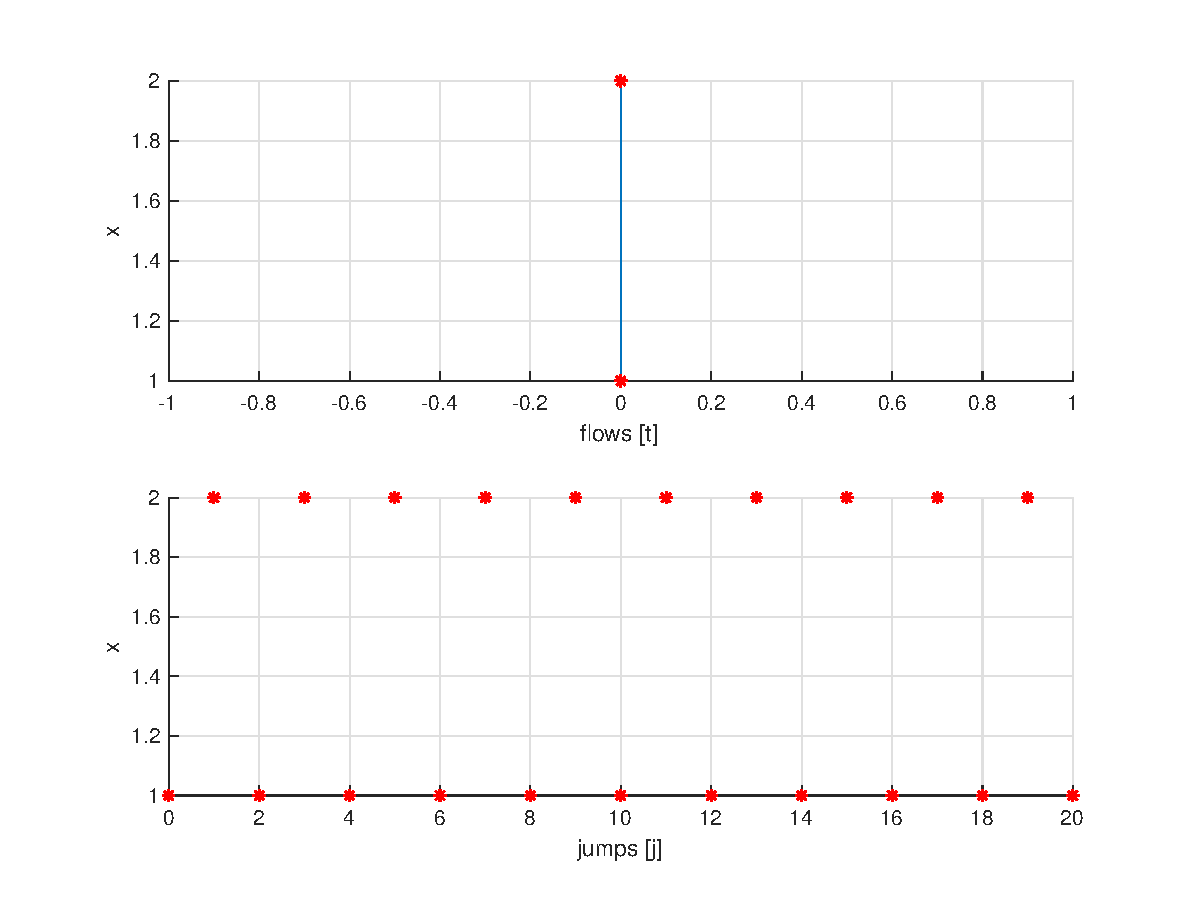
\includegraphics[width=.45\textwidth]{figures/Examples/Overlap1JumpPriority}
{
  \psfrag{flows [t]}[c]{flows [$t$]}
  \psfrag{jumps [j]}[c]{jumps [$j$]}
  \psfrag{x}[c]{$x$}
}
}
\hfill
\subfigure[Forced flows logic. \label{fig:overlap1-2}]
{
    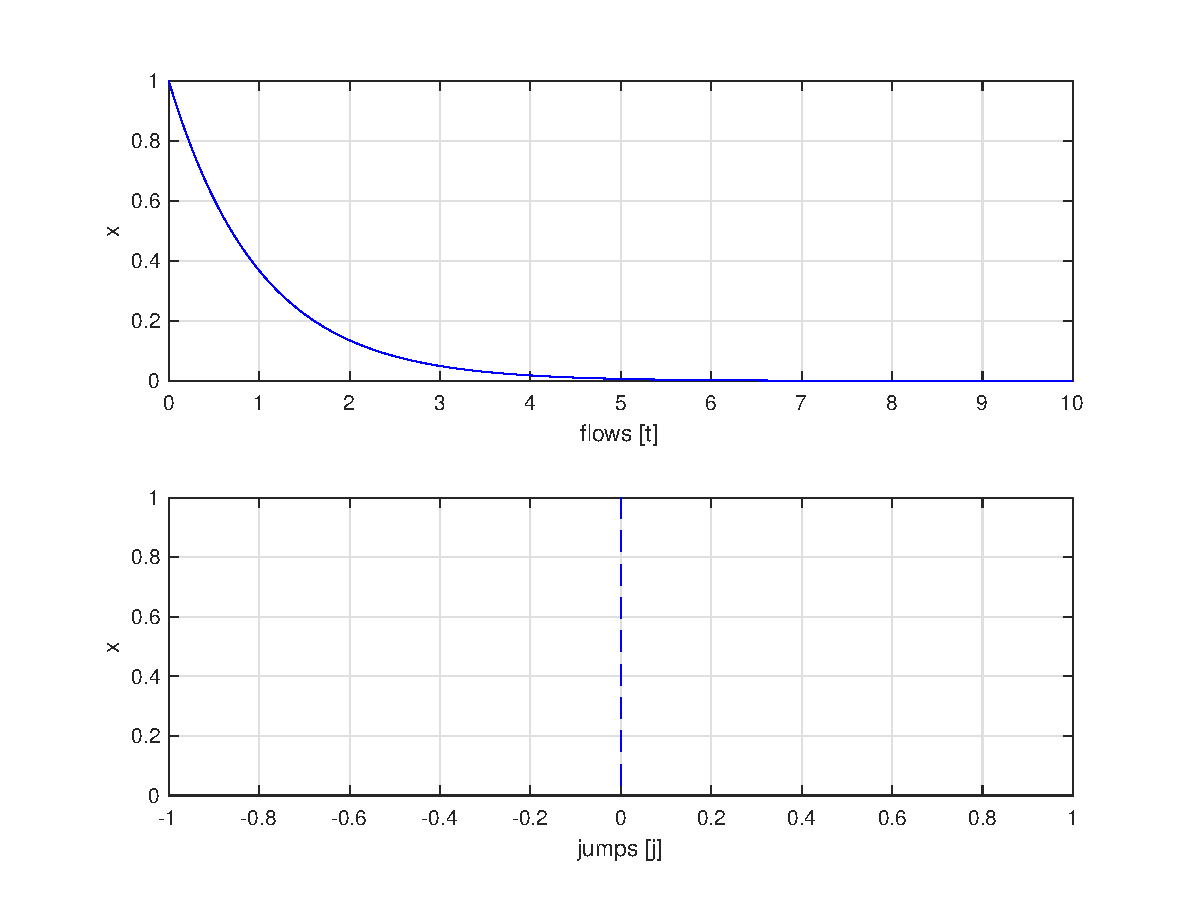
\includegraphics[width=.45\textwidth]{figures/Examples/Overlap1FlowPriority}
{
  \psfrag{flows [t]}[c]{flows [$t$]}
  \psfrag{jumps [j]}[c]{jumps [$j$]}
  \psfrag{x}[c]{$x$}
}
}
\end{center}
\caption{Solution of Example~\ref{ex:overlap1}}
\end{figure}

\begin{figure}[ht]
  \psfrag{flows [t]}[c]{flows [$t$]}
  \psfrag{jumps [j]}[c]{jumps [$j$]}
  \psfrag{x}[c]{$x$}
  \centering
\subfigure[Random logic for flowing/jumping.]{
    \includegraphics[width=.45\textwidth]{figures/Examples/Overlap1RandomPriority.eps}
\label{fig:overlap1-3}}
\subfigure[Random logic for flowing/jumping.]{
    \includegraphics[width=.45\textwidth]{figures/Examples/Overlap1TRandomPriority.eps}
\label{fig:overlap1T-1}}
\qquad
\subfigure[Random logic for flowing/jumping. Zoomed version.]{
    \includegraphics[width=.45\textwidth]{figures/Examples/Overlap1TRandomPriorityZoom.eps}
\label{fig:overlap1T-2}}
\caption{Solution of Example~\ref{ex:overlap1}}
\end{figure}

{\bf Random rule:}
A solution from $x0=1$ with $T=10,J=20$, $rule = 3$ is depicted in
Figure~\ref{fig:overlap1-3}. The solution jumps to $2$, then jumps to
$1$ and flows for the rest of the time converging to zero
exponentially.
Enlarging $D$ to
\begin{eqnarray*}
D:=  [1/50,1]\cup\{2\}
\end{eqnarray*}
causes the overlap between $C$ and $D$ to be ``thicker''.
The simulation result is
depicted in Figure~\ref{fig:overlap1T-1}
with the same parameters used in the simulation in
Figure~\ref{fig:overlap1-3}.
The plot suggests that the solution jumps several times until
$x<1/50$ from where it flows to zero.  However,
Figure~\ref{fig:overlap1T-2},
a zoomed version of Figure~\ref{fig:overlap1T-1},
shows that initially the
solution flows and that at $(t,j)=(0.2 e-3,0)$ it jumps. After the jump,
it continues flowing, then it jumps a few times, then it flows, etc.
The combination of flowing and jumping occurs while the solution
is in the intersection of $C$ and $D$, where the selection
of whether flowing or jumping is done randomly due to using $rule=3$.

This simulation also reveals that this implementation does not
precisely generate hybrid arcs. The maximum step size was set to $0.1
e-3$. The solution flows during the first two steps of the integration
of the flows with maximum step size. The value at $t=0.1e-3$ is very
close to $1$. At $t=0.2e-3$, instead of assuming a value given by the
flow map, the value of the solution is about $0.5$, which is the
result of the jump occurring at $(0.2e-3,0)$. This is the value stored
in $x$ at such time by the integrator. Note that the value of $x'$ at
$(0.2e-3,0)$ is the one given by the flow map that triggers the jump,
and if available for recording, it should be stored in $(0.2e-3,0)$.
This is a limitation of the current implementation.

The following simulations show the {\em Stop Logic block} stopping
the simulation at different events.
\begin{figure}[ht]
  \centering
  % \psfrag{flows [t]}[c]{flows [$t$]}
  % \psfrag{jumps [j]}[c]{jumps [$j$]}
  % \psfrag{x}[c]{$x$}
\subfigure[Forced jump logic and different $D$.]{
    \includegraphics[width=.45\textwidth]{figures/Examples/Overlap2JumpPriority.eps}
\label{fig:overlap2-1}}
\qquad
\subfigure[Forced flow logic.]{
    \includegraphics[width=.45\textwidth]{figures/Examples/Overlap4FlowPriority.eps}
\label{fig:overlap4-1}}
\caption{Solution of Example~\ref{ex:overlap1} with premature stopping.}
\end{figure}

{\bf Solution outside $C\cup D$:}
Taking $D = \{1\}$, a simulation starting from $x0=1$ with $T=10,J=20$, $rule = 1$ stops since the solution leaves $C\cup D$. Figure~\ref{fig:overlap2-1} shows this.

% show stopping logic by C
{\bf Solution reaches the boundary of $C$ from where jumps are not possible:}
Replacing the flow set by  $[1/2,1]$
a solution starting from $x0=1$ with $T=10,J=20$ and $rule = 2$
flows for all time until it reaches the boundary of
$C$ where jumps are not possible. Figure~\ref{fig:overlap4-1}
shows this.

Note that in this implementation, the Stop Logic is such that when the
state of the hybrid system is not in $(C \cup D)$, then the
simulation is stopped. In particular, if this condition becomes true
while flowing, then the last value of the computed solution will not
belong to $C$. It
could be desired to be able to recompute the solution so that its last
point belongs to the corresponding set. From that point, it should be
the case that solutions cannot be continued.

For MATLAB/Simulink files of this example, see \IfSAE{Examples/Example\_\ref{ex:overlap1}}{Examples/Example\_1.8}.

\end{example}



